\chapter{Hardware Description Languages}
\label{kap:HDL}
When the integrated circuit was invented only a few transistors had to be placed on a single chip. The design and placement of the transistors was done manually. With increasing technology transistors became smaller and more could be place on one chip. The integration became more complex, and designing a chip manually was not suitable any more. The solution for this problem was the development of so called \textit{Hardware Description Languages}.\\
The purpose of those languages was to create text-based descriptions of electric circuits and synthesizing them automatically with predefined databases to a hardware layout. In the 1980s Verilog and VHDL were released, which are the two most popular HDLs.
\subsubsection{VHDL}
The \textit{Very high-speed integrated circuit Hardware Description Language} is a HDL originally developed by the US Department of Defense to document the behaviour of an ASIC. It describes logical models and electrical circuits using text files and is standardised in IEEE 1076.

\lstset{language=VHDL, tabsize=4}
\begin{center}
  \begin{tikzpicture}
    \node [fill=codebgcolor]
    {{
        \begin{tabular}{l}
\begin{lstlisting}
entity FullAdder is
	port (a, b, ci: in std_logic;
		s, co: out std_logic;
	);
end FullAdder;

architecture behaviour of FullAdder is
begin
	process (a, b, ci)
	begin
		s <= a xor b xor ci;
		co <= (b and ci) or (a and ci) or (a and b);
	end process;
end behaviour;
\end{lstlisting}
       \end{tabular}
      }};
  \end{tikzpicture}
\end{center}

\subsubsection{Verilog}
Verilog is another text-based HDL standardised in IEEE 1364. 

\lstset{language=Verilog, tabsize=4}
\begin{center}
  \begin{tikzpicture}
    \node [fill=codebgcolor,rounded corners=5pt]
    {{
        \begin{tabular}{l}
\begin{lstlisting}
module FullAdder(a, b, ci, s, co);
	input a, b, ci;
	output s, co;
	reg s, co;
	
	always @ (*)
	begin
		s <= a ^ b ^ ci;;
		co <= (b & ci) | (a & ci) | (a & b);
	end
endmodule
\end{lstlisting}
       \end{tabular}
      }};
  \end{tikzpicture}
\end{center}

\section{Differences between HDLs and Computer Programming Languages}
HDLs differ from computer programming languages like C or Java in that case, that HDLs have possibilities to describe signal strength and propagation delays of signals. As CPLs have only sequential descriptions of algorithms, HDLs also model algorithms in concurrent matter.\\
In HDLs two types of assignments exist, which are the blocking operator = as well as the non-blocking assignment \textless=. Blocking assignments are evaluated and assigned in one single step, in which the execution flow of the procedure is blocked until the assignment is completed. The non-blocking assignment evaluates the right-hand side immediately while the left-hand side is postponed until other evaluation steps in this time step are completed. The execution flow continues in that case.\cite{Sut96}
\section{Abstraction Levels}
The purpose of using different abstraction levels is to hide details which are not essential for the current view of the problem. Information that is not important is hidden in higher levels of abstraction. The different abstraction levels of HDLs are shown in figure \ref{fig:hdlabstractionlevels}.
\begin{figure}[htbp]
\begin{center}
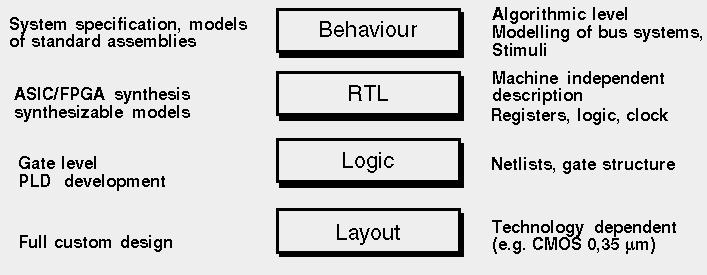
\includegraphics[width=10cm,keepaspectratio=true]{bilder/png/hdlabstractionlevels}
\caption{Abstraction levels of a HDL \cite{Ver16}}
\label{fig:hdlabstractionlevels}
\end{center}
\end{figure}
\subsection{Behavioural Level}
The behavioural level describes the behaviour of a system, regarding to its input-output relationships.\cite{Hartenstein1987}. The system is shown defining concurrent algorithms, where each of them is in a sequential manner. The behavioural level is often used to model complete systems. Also stimuli for the RTL-level are described in that level. A point to mention is the fact, that no system clock is defined and signal transitions are asynchronous with respect to the switching time.\\
It must be pointed out, that hardware descriptions in the behavioural level are simulateable, but usually not synthesizable. This means that no hardware manufacturing process can be done using only that description.\cite{Ver16}
\subsection{Register-Transfer Level}
One step down from the behavioural level the register-transfer level is used. The system complexity is broken down to combinational logic and storage elements like registers. The transfer of data between registers is defined. An explicit clock is defined, and transitions only occur in defined clock cycles. Furthermore storage elements (flip-flops) are controlled by clock cycles. The RTL is fully synthesizable.\cite{Ver16}\cite{Asic14}
\subsection{Logical Level}
The logical level, sometimes also called gate level, represents the system as netlist with storage elements and logic gates (AND, NOR, ...). The representation is done using logical links with technology-specific timing properties. Signals have only discrete logical values. In most cases the generation fo the gate netlist is done using automated synthesis tools.
\subsection{Layout Level}
To fabricate the design to a physical chip the logic level model has to be transferred to a physical model, where the exact geometric placement and the topology placement of the system has to be defined. During this process every gate and storage element is transferred to layers of metal, silicon, contacts etc.\cite{Cey96} In this level the length of wires connecting the gates can be converted proportional to propagation delays. This should be considerated for timing issues according to the clock rate.
\section{Basic Components of VHDL}
There are three basic VHDL elements. The \textit{architecture} describes the interfaces of the model. It can be compared with a single chip of a whole system. The number and naming of the interfaces is done using the \textit{port}-statement and has to be unique. The \textit{entity} describes the algorithm of the system. Each entity has to be related to at least one architecture. To exchange information between blocks the \textit{signal}-statement is used, but it is not possible to exchange information between different architectures. For more information on VHDL-elements see \cite{JuergenReichardt2013}.